\chapter{Travail réalisé}
Ce chapitre sera consacré aux solutions retenues et à leur mise en \oe uvre d'un
point de vue essentiellement technique. Chaque fonctionnalité sera séparée dans
une section propre et sera développée en suivant le schéma suivant :
\begin{itemize}
  \item Recherche et analyse
  \item Solution mise en \oe uvre
  \item 
\end{itemize}

Je n'aborderai pas ici la phase de test car je l'ai développée dans la partie
démarche méthodologique. En effet, cette phase est la même pour chaque
fonctionnalité développée. Je préfère donc me concentrer ici sur l'analyse et
les solutions apportées pour chaque fonctionnalité. %TODO lien
\section{IMS}
\subsection{Recherche et analyse}
Dans un premier temps, il m'a fallu me renseigner sur cette norme que je ne
connaissais pas du tout. Il est resortie de cette étude que les paquetages de
contenu IMS sont des archives au format standard \gloss{zip}. Or, un avantage
pour moi est que la logique de création d'une archive zip existe déjà dans
Elaastic et est utilisée pour l'export de cours au format HTML empaqueté dans
une archive zip.

Cependant, une paquetage IMS n'est pas qu'une archive zip quelquonque. Une
organisation spécifique est nécessaire à l'intérieur de cette archive. Cette
organisation est personnalisable et renseignée dans un fichier {\tt
manifest.ims} placé à la racine de l'archive. Ce fichier contient des données au
format XML décrivant l'organisation du cours empaqueté, les différentes
resources contenues dans l'archive et des méta-données relative à ce cours
(auteur, date, licence, etc.). La syntaxe de ce fichier nous permet de lier des
resources à chaque élément du cours.
Ainsi, en reprenant la structure de nos sections, sous-sections, unités dans ce
fichier manifest et en liant le contenu des unités au format HTML de notre cours
en tant que resources de cette unité, nous aurons un paquetage de contenu IMS
complet qui pourra être lu et affiché par le LMS de l'utilisateur reprenant le
contenu et les resources tel qu'il l'a rédigé dans Elaastic.

IMS GLC nous fournit également un schéma XSD pour valider la construction de ce
fichier manifest, ce qui nous permettra de vérifier que ce dernier est conforme
à la norme et que notre archive sera reconnue par les applications qui
l'utiliseront.

\subsection{Solution mise en \oe uvre}
Pour la création de l'archive zip, j'ai donc repris la logique utilisée pour
créer l'archive pour l'export au format HTML \og zippé \fg{}. Ce système utilise
des flux et des entrées pour ajouter les fichiers à l'archives. Les flux lisent
des données binaires tandis que les entrées séparent les différents fichiers de
l'archive. La logique est donc la suivante : 

On crée un {\tt ZipOutputStream}
qui sera notre flux dans lequel nous enverrons le contenu des différents
fichiers. Ensuite, on crée une {\tt ZipEntry} qui correspondra à un fichier dans
l'archive en lui passant le chemin de ce fichier à l'intérieur de l'archive. Si
des répertoires doivent être créés pour satisfaire le chemin du fichier, il le
seront automatiquement. On ajoute cette entrée au flux grâce à une méthode
{\tt newEntry()}. Puis on evoie les données correspondant au contenu du
fichier de la {\tt ZipEntry} directement dans le flux grâce aux opérateurs
flux du langage.\\

Pour la création du fichier {\tt manifest.ims}, j'ai utilisé la classe {\tt
MarkupBuilder} qui permet de créer des construire une structure de données au
format XML en spécifiant le nom, les attributs, les enfants et le contenu de
chaque élément du XML. Cette classe prend un {\tt Writer} à la construction que
j'ai instancié en tant que {\tt StringWriter}.\\

La première section du fichier manifest est la partie sur les méta-données. Cela
se traduit par la section {\tt <metadata>} du fichier manifest.\\

J'ai ensuite implémanté une structure de parcours du cours qui va remplir le
{\tt MarkupBuilder} en fonction de si nous sommes dans une section/sous-section
ou dans une unité de cours. 

Dans le cas d'une section/sous-section, le {\tt MarkupBuilder} ajoutera une
entrée {\tt <item>} dans laquelle sera ajouté le titre de la
section/sous-section et ses enfants.

Dans le cas d'une unité, le {\tt MarkupBuilder} ajoutera une entrée {\tt <item>}
dans laquelle sera ajouté simplement le titre de cette unité. Le contenu de
cette unité sera ajouté comme une entrée {\tt <resource>} dans la partie
correspondante du manifest. Toutefois, un attribut {\tt res} est ajouté à la
balise {\tt <item>}. La valeur de cet attribut est le nom de la resource
correspondant au contenu de l'unité. Cet attribut lie les deux éléments et
permettra de retrouver le contenu de l'unité lors de la lecture du paquetage par
une application tièrce.\\

Viens enfin la partie correspondant aux resources. Les resources sont les
fichiers de contenu de chaque unité de cours au format HTML. Les noms de ces
resources doivent correspondrent à ceux renseignés dans les balises {\tt <item>}
des unités de cours.\\

Une fois notre {\tt MarkupBuilder} complet, l'extraction du contenu en tant que
chaîne de caractère se fait via le {\tt StringWriter}. Avec cette chaîne
construite, nous pouvons vérifier que sa construction est correcte en la
validant avec le schéma XSD fournis par IMS GLC.

Si la construction n'est pas validée, l'export est annulé.

Si la construction est validée, l'export se poursuit. Les fichiers de contenu de
cours au format HTML sont ajoutés à l'archive zip ainsi que les images
référencées dans ces contenus.\\

Maintenant que nous avons une archive complète, nous pouvons la retourner à
l'utilisateur dans une réponse HTTP en précisant {\tt application/zip} comme
{\tt ContentType}.

\section{WebDAV}
\subsection{Recherche et analyse}
Comme pour l'IMS Content Packaging, il m'a d'abord fallu me renseigner sur ce
qu'était WebDAV.

WebDAV est une extension du protocole HTTP. Il comprend un ensemble de nouvelles
méthodes qui s'utilisent avec le protocole HTTP. Ces méthodes permettent de
créer, modifier et/ou supprimer des fichiers sur le serveur WebDAV. Elles
permettent aussi de consulter/modifier les propriétés de ces fichiers. Un
système de gestion de version est aussi dispoonible via des commande de verrou
sur les fichiers pour protéger des écritures concurentes.

Avant tout, j'ai cherché si un plugin Grails n'existait pas déjà gérant les
échange WebDAV. Et il s'est avéré qu'un tel plugin existe sur un dépôt Maven. Or
nous utilisons le système de dépendence de Maven pour les dépendences de notre
projet. Ce plugin s'appelle Sardine, est codé en Java et est disponible sur
GitHub\footnote{\url{https://github.com/lookfirst/sardine}}. J'ai donc enquêté
sur la fiabilité de ce plugin en recherchant des avis et d'éventuels manques vis
à vis du protocole. La fréquence des commits et les différents avis que j'ai pu
receuillir m'ont convaincu quant à l'utilisation de ce plugin.

\subsection{Solution mise en \oe uvre}
Pour cette fonctionnalité, j'ai développé un service Grails qui interface le
plugin Sardine et fournit des méthodes pour créer, mettre à jour, supprimer
des fichiers sur un serveur WebDAV.

Pour tester le bon fonctionnement de cette fonctionnalité, j'ai également mis en
place un serveur WebDAV sur ma machine.\\

Cependant, d'autres fonctionnalités prioritaires étaient à développer et
intégrer avant celle-ci. Mon travail est donc dans une branche du git en
attendant d'être complété et intégré au projet.

\section{Artifact}
\subsection{Recherche et analyse}
Le besoin d'avoir des artéfacts vient du fait que la tranformation d'un cours en
format de sortie pour l'utilisateur final est trop long pour une utilisation
fluide de l'application. Ce temps de transformation sera encore plus évident
quand nous aborderons la partie sur la diffusion d'un cours.

Un artéfact est une version précise d'un cours, transformé dans un format
particulier. Le nom {\tt Artifact} correspond à la collection/table qui sera
stockée en base. Ce système de persistene permettra de faire office de cache et
de retourner à l'utilisateur une version tranformée du cours plus rapidement.

Il est également nécessaire d'ajouter une contrainte d'unicité sur les artifacts
afin de garder l'intégrité des données et n'avoir qu'un document à retourner à
l'utilisateur pour une version de cours et un format donné. Cette contrainte
portera donc sur le cours, sa version et le format de l'artéfact.

\subsection{Solution mise en \oe uvre}
Pour la mise en place de cette solution, il y a deux étapes.\\

La première étape est de créer la classe du domaine {\tt Artifact} qui
correspond aux champs qui seront stockés en base et aux contraintes sur ces
paramètres comme la contrainte d'unicité exposée plus haut. Ensuite, j'ai créé
une classe {\tt ArtifactService} de service Grails qui assure les échanges
transactionnels avec la base de données. Cette classe suit les mécaniques
CRUD\footnote{{\bf C}reate {\bf R}ead {\bf U}padte {\bf D}elete} de
Grails. Elle fournit une méthode {\tt save} pour ajouter une nouvelle entrée et
des méthodes {\tt findBy} pour récupérer un artifact en fonction d'une ou
plusieurs des conposantes de la contrainte d'unicité.\\

La deuxième étape est d'ajouter une vérification de l'existance d'un artifact
avant l'export d'un cours. La logique de ce cache avec les artéfacts est la
suivante : Lorsqu'un utilisateur demande l'export d'un cours dans un format
particulier, si un artéfact correspondant à ce cours, dans cette version et dans
ce format existe en base, on peut directement le renvoyer à l'utilisateur avec
le bon {\tt ContentType}. Par contre, si aucun artéfact ne correspond en base,
on doit effectuer la transformation. Une fois cette tranformation effectuée, on
stoque le binaire généré en base avec le cours, sa version et le format
correspondant. Ainsi, à la prochaine demande, l'élément sera dans un \og cache
\fg{} et récupéré directement.\\

Le développement de cette deuxième partie a montré une dupplication de code avec
l'intégration de ce système de cache. En effet, le code est le même pour chaque
exporteur. Nous avons donc mis en place un système plus générique au niveau des
exporteurs. La factorisation de ces exporteurs nous a permis d'isoler une classe
abstraite principale {\tt CourseExporter} et différentes implémentations : {\tt
ImsCourseExporter}, {\tt PdfCourseExporter}, {\tt
OnlineSlideShowCourseExporter}, etc. De plus, nous avons mis en place une \og
factory \fg{} pour la création de ses exporters. Cette factory ajoute en
fonction des besoins des décorateurs pour l'export au format zip ou la mise en
cache. Ces décorateurs implémentent eux aussi la classe abstraite {\tt
CourseExporter} Ainsi, nous nous retrouvons avec une seule classe {\tt
ZipCourseExporter} et une seule calsse {\tt CacheCourseExporter}. En les
connectant, on peut metter en cache et/ou empaqueter dans une archive zip
n'importe quel format d'exportation avant de le livrer à l'utilisateur.

\section{Diffusion}
\subsection{Recherche et analyse}
La possibilité de diffuser un cours est une des fonctionnalités capitales
d'Elaastic. Cette diffusion permettra aux étudiants d'accéder à des versions en
\og lecture seule \fg{} de ces cours dans les différents formats disponible à
l'exportation. Une diffusion correspondra donc à un cours dans une version
particulière. Avec ce système en place, on peut rapidement immaginé une charge
importante sur le serveur lorsque plusieurs groupes d'étudiants voudront
récupérer la même version d'un cours en particulier. C'est avec des échelles
comme celle-là que l'importance du système de cache avec les artéfacts se
justifie pleinement.

Les diffusions seront stockées en base correspondant à un cours, sa version, un
nom d'affichage, un nom normalisé pour l'URL et un type de diffusion. Pour
l'instant, nous n'avons défini qu'un seul type de diffusion : {\tt
ELAASTIC\_SIMPLE}. C'est celui mentionné d'ici là dans ce document. Il permet de
récupérer un cours dans une version particulière et dans les formats disponibles
à l'exportation.

\subsection{Solution mise en \oe uvre}
Mon travail sur cette fontionnalité a principalement été de mettre une interface
sur \og externe \fg{} à l'éditeur pour obtenir un cour dans un des formats
d'exportation. J'ai donc créé un contrôleur Grails, {\tt PlayerController}, qui
se charge de formater le sortie de la diffusion en fonction de la requête de
l'utilisateur. Avec se contrôleur, j'ai ajouté les entrées correspondantes dans
le fichier {\tt UrlMapping} de Grails et j'ai créer une vue pour lister les
exports difsponibles dans cette diffusion. L'URL est pensée pour être \og human
readable\footnote{Facilement lisible par un être humain} \fg{}. Elle se
construit comme suit : {\tt http://<url de l'application>/<utilisateur>/<nom de cours
normalisé>}. La figure \ref{fig:diffusion} illustre une partie de la vue qui
liste les formats dispoibles. Les liens sur cette vue redirigent vers les
exporteurs correspondant au format choisi.

\begin{figure}[h]
  \centering
  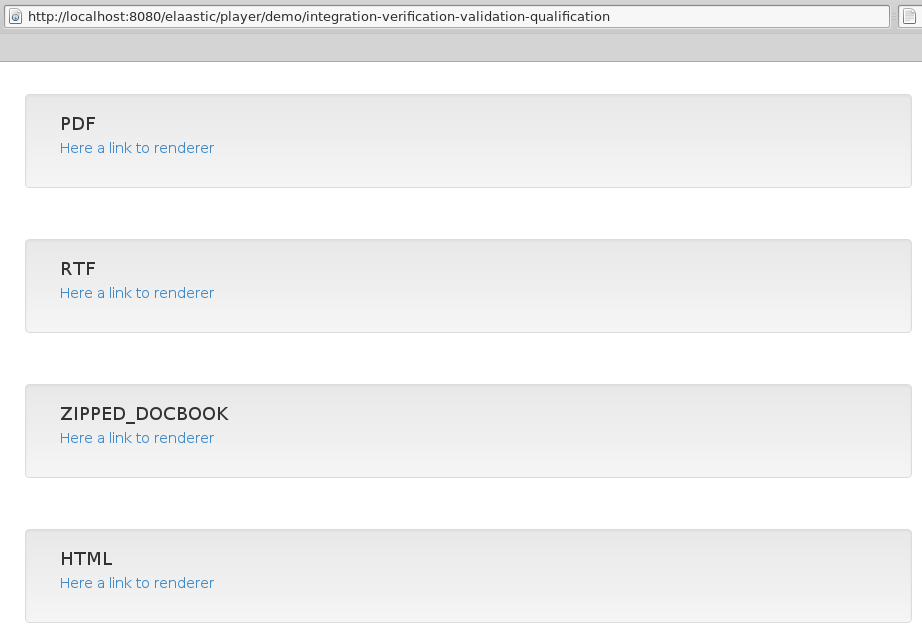
\includegraphics[width=15cm]{images/diffusion.png}
  \caption{Une diffusion de type {\tt ELAASTIC\_SIMPLE}}
  \label{fig:diffusion}
\end{figure}

\section{Question intéractive}
\subsection{Recherche et analyse}
Là encore, le langage Moodle GIFT a été une découverte pour moi. il m'a fallu
lire la documentation pour apprivoiser la syntaxe et les possibilités de ce
langage. Cependant, Franck utilisait déjà un analyseur de code Moodle GIFT dans
Tsaap-Notes. Il l'a extrait et en a fait un plugin Grails -- appellé
Tsaap-Questions -- que j'ai pu intégré à Elaastic. Ce plugin retourne un graphe
d'objet Java correspondant à un {\tt Quiz} composé de {\tt Question}s,
elles-même composés de {\tt TextBlock}s et d'{\tt Answer}s. Il m'a également
guidé à travers ces concepts pour comprendre comment récupérer ce qui
m'intéressait dans ces questions et me donner des pistes pur le rendu de ces
questions dans les différents formats.\\

Par ailleurs, ces différents formats ne sont pas tous \og intéractifs \fg{}. Par
exemple, le rendu ne pourra pas être le même pour un diaporama HTML, où les
questions peuvent être des formulaires et les réponses retraitées pour établir
des statistiques ou des retour pour les utilisateurs, que pour un PDF où chaque
étudiant répondra de son côté à ces questions sans intéraction avec les autres
étudiants de la promotion. Il a fallu donc différencier les types \og statiques
\fg{} des types \og dynamiques \fg{}. La séparation s'est faite comme suit :
\begin{itemize}
  \item Types dynamiques :
	\begin{itemize}
	  \item Diaporama HTML ;
	  \item HTML empaqueté dans un zip (l'intéraction se fera via une API REST) ;
	  \item IMS Content Packaging (le rendu étant du HTML, le fonctionnement est
		le même que pour l'HTML zippé).
	\end{itemize}
  \item Types statiques 
	\begin{itemize}
	  \item Docbook ;
	  \item PDF ;
	  \item RTF.
	\end{itemize}
\end{itemize}

\subsection{Solution mise en place}
Pour rendre la saisie de question possible, j'ai ajouté un type d'élément de
cour. Ces types sont renseignés dans l'énumération {\tt ElementType}. Chaque
élément de cour est de type {\tt ElementType}. La distinction se fait au niveau
des exporteurs qui traitent les sections/sous-sections différemment des unités
et maintenant des questions. Ainsi, lors de l'export d'un élément de type {\tt
QUESTION}, le plugin Tsaap-Questions est appellé pour convertir cette question
en graphe d'objets, puis ces objets sont analysés et transformés en :
\begin{itemize}
  \item un formulaire HTML pour les types dynamiques ;
  \item une liste à puce pour les formats statiques.
\end{itemize}



